
%%%%%%%%%%%%%%%%%%%%%%% file typeinst.tex %%%%%%%%%%%%%%%%%%%%%%%%%
%
% This is the LaTeX source for the instructions to authors using
% the LaTeX document class 'llncs.cls' for contributions to
% the Lecture Notes in Computer Sciences series.
% http://www.springer.com/lncs       Springer Heidelberg 2006/05/04
%
% It may be used as a template for your own input - copy it
% to a new file with a new name and use it as the basis
% for your article.
%
% NB: the document class 'llncs' has its own and detailed documentation, see
% ftp://ftp.springer.de/data/pubftp/pub/tex/latex/llncs/latex2e/llncsdoc.pdf
%
%%%%%%%%%%%%%%%%%%%%%%%%%%%%%%%%%%%%%%%%%%%%%%%%%%%%%%%%%%%%%%%%%%%


\documentclass[runningheads,a4paper]{llncs}

\usepackage{amssymb}
\setcounter{tocdepth}{3}
\usepackage{graphicx}

\usepackage{url}
\urldef{\mailsa}\path|{alfred.hofmann, ursula.barth, ingrid.haas, frank.holzwarth,|
\urldef{\mailsb}\path|anna.kramer, leonie.kunz, christine.reiss, nicole.sator,|
\urldef{\mailsc}\path|erika.siebert-cole, peter.strasser, lncs}@springer.com|    
\newcommand{\keywords}[1]{\par\addvspace\baselineskip
\noindent\keywordname\enspace\ignorespaces#1}

\begin{document}

\mainmatter  % start of an individual contribution

% first the title is needed
\title{On the liability of TOR Exit Relay operators}

% a short form should be given in case it is too long for the running head
\titlerunning{}

% the name(s) of the author(s) follow(s) next
%
% NB: Chinese authors should write their first names(s) in front of
% their surnames. This ensures that the names appear correctly in
% the running heads and the author index.
%
\author{Alessio Trivisonno}
%
\authorrunning{}
% (feature abused for this document to repeat the title also on left hand pages)

% the affiliations are given next; don't give your e-mail address
% unless you accept that it will be published
\institute{University of Trento}

%
% NB: a more complex sample for affiliations and the mapping to the
% corresponding authors can be found in the file "llncs.dem"
% (search for the string "\mainmatter" where a contribution starts).
% "llncs.dem" accompanies the document class "llncs.cls".
%

\toctitle{}
\tocauthor{}
\maketitle


\begin{abstract}
The abstract should summarize the contents of the paper and should
contain at least 70 and at most 150 words. It should be written using the
\emph{abstract} environment.
\keywords{Tor, Exit Node, Operator, ISP, Internet Service Provider, Liability}
\end{abstract}


\section{Introduction}

\section{Background}

\subsection{What is TOR}

Tor is a free and open source software aimed to enable anonymous communication on the web. It is one the most used and secure \textit{Privacy Enhancing Technology} that is available now.\footnote{Although the technology is very strong and secure there are still many attacks that can undermine the anonymity of the Tor users} We can find it in the same class as VPNs, Proxies and DNS Bypass. However it is the only technique that can truly ensure your anonymity on the web. For this reason Tor has become more and more popular during these years, especially in countries where censorship is most suffered. Today Tor is used on average by 2 Million users every day.

The name Tor stands for ``The Onion Router`` 
which is the technology at the core of this software.


The Onion Routing is a networking mechanism that ensures encryption and 
anonymity in a communication between two endpoints. The connection between 
endpoints is routed along an encrypted chain where every node in the chain is 
called a relay. Each relay has the knowledge of only the previous and the 
following nodes in the chain. This makes the complete picture of the communication hidden from anyone. \cite{CCDCOF}


\subsection{How It Works}
The Tor architecture is composed of basically three entities: 
\begin{itemize}
    \setlength\itemsep{1em}
    \item The Directory Servers
    \item Middle Relays
    \item Exit Relays
\end{itemize}
The Directory Servers advertise the entry points of the Tor Network to the client while the network
itself if composed by Middle Relays and Exit Relays. 
Tor creates a circuit starting from the end user to the destination that jumps on 
different hops during its path and at each jump the intermediate packet is encapsulated 
into an additional layer of encryption. From the moment that the request of the end user 
enters the network is jumps randomly on a set of Middle Relays before reaching the Exit Relay. 
Exit relays are the points in which the request of the end user makes the last step towards 
the final destination. See Fig \ref{fig:fig_tor_arch}

\begin{figure}[]
    \center{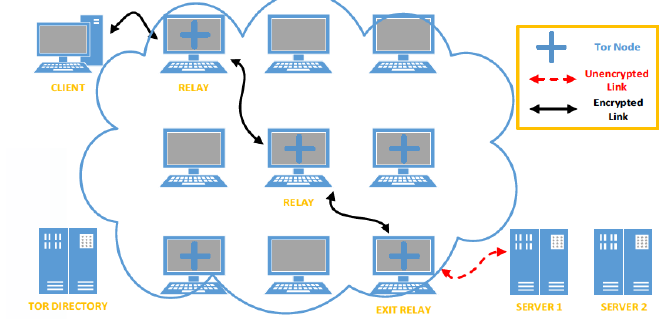
\includegraphics[width=0.5\textwidth]
        {./figures/tor_arch.png}}
        \caption{ Tor architecture}
        \label{fig:fig_tor_arch}
\end{figure}

All the relays in the network are run by individual volunteers or organizations and the technology 
relies on this to guarantee the anonymity.

As shown in Fig \ref{fig:fig_tor_arch} the connection between client/relay and relay/relay is encrypted
and does not cause any problems to the operator. The Exit Relays instead, are the one that carry out the 
last-mile communication. They are the most exposed part of the network, since the communication between
the client and the server is at this stage unencrypted, making the request look like as it is the 
Exit Relay which is originating that traffic. 

\section{For what Tor is used for}
Tor has been developed with the idea that anyone should be able to express their belief without beeing monitored by others, not even governments. Among its main usage we can find privacy protection for individual that are unwilling to give away their navigation data to ISPs. In the business filed Tor is used to ensure confidentiality and for doing research on competitors without leaving traces. Similarly Tor can be used for intelligence gathering by government's body like U.S. Navy, in fact the very technology of Onion Routing was developed by them. It can also be used to protect the identity of sources for journalists, like whistleblowers. And It can also help activists to report abuse or organize meetings, as it happened during the Egyptian Revolution of 2011. \cite{WASH_715}

\begin{figure}[]
    \center{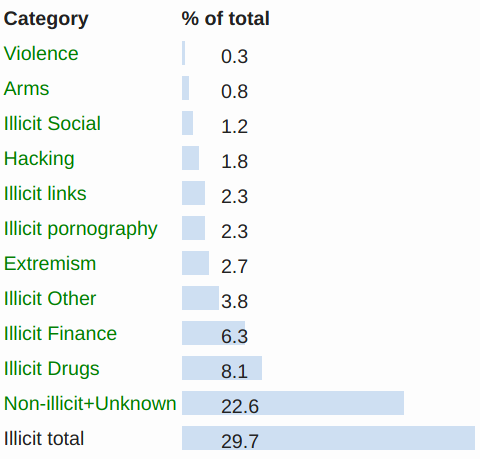
\includegraphics[width=0.5\textwidth]
        {./figures/tor_illicit.png}}
        \caption{Web-Based Onion Services in February 2016 (Source Wikipedia.org)}
        \label{fig:fig_tor_ill}
\end{figure}

Beside that Tor has been accused to be full with criminal activity, especially regarding child pornography and drug dealing. As shown in figure \ref{fig:fig_tor_ill} the amount of illicit activity percentage on the overall onion services is high (almost 30\%). For example famous were the cases of the sites PlayPen and SilkRoad that led to the incarceration of many users and maintainer of those sites. 

\section{The problem: Liability of Tor Exit Relays Operators}
Since the Tor Exit Relay Operators are the one that carry on the \textit{last mile communication} they are the one that are most exposed in terms of legal actions. In fact if from their server transit a request from a generic Tor user for a site that hosts child pornography, such request cannot be distinguished from the normal traffic of the operator. 
Exit Relays behave in the same way normal relay does, they remove the source ip address and replaces it with its own ip address as a source, lastly it forwards the request to the next hop. In this case the last hop is the final destination and as shown in Fig. \ref{fig:fig_tor_arch} the communication between the Exit Relay and the destination server is no more encrypted by the Tor protocol \footnote{The communication can still be encrypted at application level with HTTPS but the source and destination ip address are no longer anonymised}. 
TODO: Company Terms of Service, like Aruba

\section{The case Austrian Regional Crime Court vs William Weber}
In this section I will present the case of Austrian regional criminal court in Graz vs. W. Weber. This case sees W.Weber, a tor exit node operator being sentenced by the court for aiding the distribution of child pornography. I will discuss the case and talk about the reason why he was held accountable and what where the court motivation for that.

On June 30th 2014 William Weber a Tor Exit Node Operator was sentenced to 3 months of jail and 3 years of probation for helping the distribution of child pornography on through his server.

As we discussed in the previous paragraph, Tor Exit Node Operators are the one that are most exposed in terms of criminal liability since they supply their internet access point and their unique IP address to the Tor community.

The main reason why the court judged W.Weber liable of aiding the distribution of child pornography was that he was intercepted while talking to an anonymous person on the web about the possibility of hosting child pornography on his server. He said: 
\begin{quote}
    \textit{ "You can host 20TB child porn with us on some encrypted HDD”[...] “You can host child porn on our servers” [...] “If you want to host child porn ... I would use Tor.”}
\end{quote}
That showed to the Court that not only was he at least aware that his Tor node could have been used to do distribute child pornography, but also he does not disapprove that.
However he declared on his blog that this conversation was used out of context and that he was just talking hypothetically. 
Despite that, he was found guilty because (as stated by Huťko \cite{HUSOVEC}):
\begin{quote}
\textit{
    The Austrian Court found that this activity may lead to criminal liability for aiding and abetting of a crime of distribution of child pornography when coupled with other circumstances.}
\end{quote}
The other circumstances that invalidated the \textit{mere conduit} safe harbour were these very transcript. In fact as stated by Art.12 of the eCommerce Directive 
\begin{quote}
    \textit{1. Where an information society service is provided that consists of the transmission in a communication network of information provided by a recipient of the service, or the provision of access to a communication network, Member States shall ensure that the service provider is not liable for the information transmitted, on condition that the provider:\\
(a) does not initiate the transmission;\\
(b) does not select the receiver of the transmission; and\\
(c) does not select or modify the information contained in the transmission.}
\end{quote}

Also it is to say that forensic experts have reconstructed some images depicting pornographic acts of children. However he could not be found guilty since there was no evidence that these picture were effectively downloaded by him or by the the automatic caching mechanism. And he was by far protected by the article 12 section 2 of the eCommerce Directive for these evidence:

\begin{quote}
    \textit{2. The acts of transmission and of provision of access referred to in paragraph 1 include the automatic, intermediate and transient storage of the information transmitted in so far as this takes place for the sole purpose of carrying out the transmission in the communication network, and provided that the information is not stored for any period longer than is reasonably necessary for the transmission.}
\end{quote}

But, since he was intercepted having that conversation with the anonymous user, he was actively collaborating with the intent of doing illegal activities with that person. That invalidated the liability exemption from "mere conduit" considering the Recital 44 of the Directive:

\begin{quote}
    \textit{
(44) A service provider who deliberately collaborates with one of the recipients of his service in order to undertake illegal acts goes beyond the activities of "mere conduit" or "caching" and as a result cannot benefit from the liability exemptions established for these activities.}
\end{quote}

At the end of this first litigation he decided to do not go in further trials and accept the sentence.

This decision demonstrates that Tor Exit Node Operators should be very cautious when operating their activity not only from the technology prospective, but also from the legal one. However as cited in \cite{HUSOVEC} \textit{we should be really careful in keeping the standard of "deliberate collaboration" very high, otherwise it might be easy to criminalize Tor Exit Nodes operators}. . Criminalizing the Tor operators would be very easy in countries \textit{with less legitimate criminal offences such as anti-state propaganda crimes} \cite{HUSOVEC}. Without their valuable work the whole anonymity network phenomena would not exist. They in fact operate in one of the most crucial point of the architecture, they connect the anonymous world with the real world, without that connection the anonymity world has no point to exist.

However this sentence has not to be considered as a sentence against Tor. Tor is still perceived as an important tool to ensure privacy and secrecy, as stated by  Shubert in the Constitudional Court who said that \textit{"privacy and especially the secrecy of communication on the Internet have to be protected"} and that the legality of Tor should not be challenged. \cite{PCW}


\section{Liability of Internet Service Providers for Copyright Infringement}
In this section I will present a similar scenario but in the case of copyright infringement. I will discuss the mere conduit safe harbor that can be applied to ISP in case of copyright infringement correlating the it with court decisions. I will also discuss weather a tor operator can be considered an ISP. This in correlation with the Directive 2000/31/EC of the European Parliament and of the Council of 8 June 2000.

\section{The situation in Italy}
In this section I will present how in Italy is handled the liability of ISP illustrating some examples on court decision, as the sentence n. 54946/2016 of the Corte di Cassazione. And also I will discuss the d.lgs 70/2003, with particular interest to art 14, art 15 and art 16.

\section{Conclusion}
\blindtext[3]



\begin{thebibliography}{9}

\bibitem{CCDCOF}
Emin \c{C}alı\c{s}kan, Tom\'{a}\u{s} Min\'{a}rik, Anna-Maria Osula (2015).
\textit{Technical and Legal Overview of the 
Tor Anonymity Network}.\\
NATO Cooperative Cyber Defence Center of 
Excellence, Tallin, Estonia

\bibitem{WASH_715}
    Keith D. Watson. (2012)
    \textit{ THE TOR NETWORK: A GLOBAL INQUIRY INTO THE LEGAL STATUS OF ANONYMITY NETWORKS . }
    Washington University Global Studies Law Review

\bibitem{EFF_PLAYPEN}
    Electronic Frontier Foundation\\
    \textit{The Playpen Cases: Frequently Asked Questions}
    link: https://www.eff.org/it/pages/playpen-cases-frequently-asked-questions\\
    date of last visit: "03/04/2019"
    
    \bibitem{HUSOVEC}
    Huťko´s Technology Law Blog\\
    \textit{Austrian Court Sentenced a Tor Exit Node Operator}
    link:     http://www.husovec.eu/2014/07/austrian-court-sentenced-tor-exit-node.html
    date of last visit: "12/04/2019"
    
    \bibitem{PCW}
    Loek Essers, PC WORLD\\
    \textit{Tor exit node operator convicted of abetting spread of child porn}
    link:         https://www.pcworld.com/article/2452320/tor-exit-node-operator-convicted-of-abetting-spread-of-child-porn.html
    date of last visit: "12/04/2019

\end{thebibliography}


\end{document}